% Layout adapted from the research memo shown in Lecture 1, sized for A4.
\documentclass[a4paper,10pt]{article}
\usepackage[margin=18mm,footskip=9mm]{geometry}
\usepackage{iftex}
\ifPDFTeX
  \usepackage[T1]{fontenc}
  \usepackage[utf8]{inputenc}
  \usepackage[scaled=0.96]{helvet}
  \renewcommand{\familydefault}{\sfdefault}
\else
  \usepackage{fontspec}
  \setmainfont{texgyreheros}[Extension=.otf,
    UprightFont=*-regular, BoldFont=*-bold,
    ItalicFont=*-italic, BoldItalicFont=*-bolditalic]
\fi
% For Chinese, set this switch true and compile with --engine xelatex.
\newif\ifChineseMemo
\ChineseMemofalse
\ifChineseMemo
  \ifPDFTeX
    \PackageError{finance-memo}{Chinese text requires XeLaTeX or LuaLaTeX}{}
  \else
    \usepackage[UTF8,fontset=fandol]{ctex}
    \renewcommand{\familydefault}{\sfdefault}
  \fi
\fi
\usepackage{booktabs,graphicx,xcolor,caption,xurl,fancyhdr}
\definecolor{MemoBlue}{HTML}{203E70}
\definecolor{MemoRule}{HTML}{B9C8DF}
\usepackage[colorlinks=true,linkcolor=MemoBlue,urlcolor=MemoBlue]{hyperref}
\captionsetup{font=small,labelfont=bf,skip=4pt}
\setlength{\parindent}{0pt}
\setlength{\parskip}{5pt}
\pagestyle{fancy}
\fancyhf{}
\renewcommand{\headrulewidth}{0pt}
\renewcommand{\footrulewidth}{0.3pt}

\newcommand{\ReportTitle}{AMD FY2026 Q3: Underperform, target price \$297}
\newcommand{\ReportType}{EARNINGS UPDATE}
\newcommand{\ReportDate}{2026-11-15}
\newcommand{\DataDate}{2026-11-03 23:00:17 UTC}
\newcommand{\ReportScope}{Quarter ended 2026-09-26 (CY2026Q3); trigger filing 0000002488-26-000191}
\newcommand{\TeamName}{Semis Coverage (coursework)}
\newcommand{\DeskName}{AI semiconductor supply chain}
\newcommand{\ReportAuthor}{Coursework analyst (AI-assisted workflow)}
\newcommand{\Coverage}{NVDA, AMD, INTC, AVGO, MRVL, MU, AMAT}
\newcommand{\KeyFinding}{Revenue \$13.4bn (16.0\% q/q); target price \$297 vs last close \$483.90 (-38.6\%).}
\fancyfoot[L]{\scriptsize\TeamName}
\fancyfoot[R]{\scriptsize\ReportType}

\begin{document}
\begin{minipage}[t]{0.70\textwidth}
\vspace{0pt}
{\small\ReportDate}\par\medskip
{\color{MemoBlue}\hrule height 0.5pt}\smallskip
{\large\ReportType}\par
{\LARGE\bfseries\ReportTitle}\par\medskip
\ReportScope
\end{minipage}\hfill
\begin{minipage}[t]{0.23\textwidth}
\vspace{0pt}\raggedleft
\colorbox{MemoBlue}{\parbox[c][19mm][c]{0.86\linewidth}{\centering\color{white}\bfseries\TeamName}}\par\medskip
\DeskName
\end{minipage}
\par\bigskip
{\color{MemoBlue}\hrule height 0.5pt}\medskip
{\large\KeyFinding}\par\bigskip

\begin{minipage}[t]{0.61\textwidth}
\vspace{0pt}\raggedright
\setlength{\parskip}{4pt}
\textbf{Summary}\par
See key points and full note below. Figures are generated by code from SEC filings; prose is AI-drafted and human-approved.
\end{minipage}\hfill
\begin{minipage}[t]{0.36\textwidth}
\vspace{0pt}\small
% Author these non-floating wrappers separately. Use \captionof{table/figure},
% then a description and \input/\includegraphics of generated content.
\IfFileExists{sections/tables.tex}{\captionof{table}{Key data, FY2026 Q3}\label{tab:key-data}
{\footnotesize Reported figures for the quarter ended 2026-09-26 (CY2026Q3) from SEC XBRL facts; NTM, DCF and target price are model outputs. US\$.\par}
\begin{tabular}{@{}lr@{}}
\toprule
Item & Value \\
\midrule
Revenue (quarter) & \$13.4bn \\
Revenue q/q & 16.0\% \\
Revenue y/y & 44.7\% \\
Gross margin & 53.9\% \\
Operating margin & 21.2\% \\
Diluted EPS & \$1.46 \\
Free cash flow & \$0.6bn \\
\midrule
NTM revenue (model) & \$72.6bn \\
NTM EPS (model) & \$9.72 \\
DCF value / share & \$195.37 \\
Peer EV/Sales (median) & 16.3x \\
Last close & \$483.90 \\
Target price & \$297 \\
Upside & -38.6\% \\
Rating & Underperform \\
\bottomrule
\end{tabular}

}{
  \textbf{Key data}\par
  [Insert a compact checked table, including units and periods.]
}
\medskip
\IfFileExists{sections/figures.tex}{\captionof{figure}{Quarterly revenue, reported and forecast}\label{fig:revenue}
{\footnotesize Solid: reported (SEC XBRL, fiscal quarters). Hatched: model forecast from this case's assumptions. US\$ bn.\par}
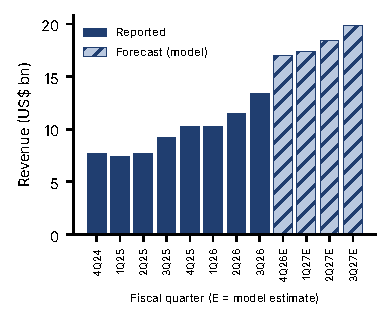
\includegraphics[width=\linewidth]{../../output/figures/AMD-0000002488-26-000191-r2/revenue.pdf}
}{
  \textbf{Supporting chart}\par
  [Insert a chart with readable labels, units, and a source note.]
}
\end{minipage}
\par\bigskip



\par\smallskip\textbf{\color{MemoBlue}Key points}\par

\begin{itemize}\setlength{\itemsep}{1pt}
\item \textbf{Reported:} FY2026 Q3 (calendar CY2026Q3, quarter ended 2026-09-26) revenue was \$13.4bn, up 44.7\% year on year and 16.0\% quarter on quarter; diluted EPS was \$1.46.
\item \textbf{Company guidance:} management guides next-quarter revenue to about \$17.0bn and non-GAAP gross margin to about 55.0\%: “For the fourth quarter of 2026, AMD expects revenue to be approximately \$17 billion, plus or minus 3\%.” “Non-GAAP gross margin is expected to be approximately 55\%.”
\item \textbf{Our forecast:} we model FY2026Q4 revenue of \$17.0bn (anchored on the guidance midpoint) and EPS of \$2.26; next-twelve-month revenue is \$72.6bn and EPS \$9.72.
\item \textbf{Our judgment:} the growth story is strong, but at \$483.90 the shares already discount far more than our cash-flow model supports. Our blended target of \$297 implies -38.6\% versus the last close, which maps to Underperform under the policy bands.
\end{itemize}

\par\smallskip\textbf{\color{MemoBlue}Results}\par

All figures in this section are reported results from the FY2026 Q3 10-Q; the financial figures are derived by code from SEC XBRL data, and quoted text is taken from the 10-Q.

\begin{itemize}\setlength{\itemsep}{1pt}
\item Revenue: \$13.4bn (44.7\% year on year, 16.0\% quarter on quarter); trailing-twelve-month revenue \$45.4bn.
\item GAAP gross margin: 53.9\%. The company attributes the year-on-year improvement to mix: “Gross margin was 54\% and 52\% for the three months ended September 26, 2026 and September 27, 2025, respectively, where the increase was driven by a favorable product mix, including higher Data Center segment revenue.”
\item GAAP operating margin: 21.2\%.
\item Net income: \$2.4bn; diluted EPS \$1.46. Reported earnings include two large one-off items that act in opposite directions. On the tax line, the 10-Q states: “In addition, the tax benefit for the three and nine months ended September 26, 2026 also included a discrete tax benefit related to stock-based compensation of \$772 million and \$918 million, respectively.” In other income (expense), it states: “During the three and nine months ended September 26, 2026, the Company recorded a noncash charge of \$1.2 billion, primarily related to a loss from remeasurement of the warrant liability based on the change in fair value of the warrants within Other income (expense), net.” Our judgment: the discrete tax benefit raises reported EPS and the noncash warrant charge lowers it. The 10-Q does not give the after-tax effect of the warrant charge, so the net effect of the two items on the recurring run rate cannot be determined from the filing; we assess recurring earnings excluding both items rather than from reported EPS.
\item Free cash flow (operating cash flow less capital expenditure): \$0.6bn, held back by a build in inventories and receivables.
\item Net cash at quarter end: \$8.7bn.
\end{itemize}

\par\smallskip\textbf{\color{MemoBlue}Guidance and outlook}\par

Company guidance (quoted from the earnings release):

\begin{itemize}\setlength{\itemsep}{1pt}
\item Revenue: “For the fourth quarter of 2026, AMD expects revenue to be approximately \$17 billion, plus or minus 3\%.”
\item Margin: “Non-GAAP gross margin is expected to be approximately 55\%.” Note that this is a non-GAAP measure; our model forecasts GAAP gross margin, which runs below the non-GAAP figure because of acquisition-related amortization and stock-based compensation in cost of sales.
\item Demand commentary: “we expect growth to accelerate further in the fourth quarter as we scale Helios and ‘Venice’ production” and “Our fourth-quarter outlook reflects accelerating revenue and earnings growth, driven by strong demand across our Data Center portfolio.”
\end{itemize}

Our forecasts (from code, using our assumptions): FY2026Q4 revenue of \$17.0bn, essentially at the guided \$17.0bn midpoint, and EPS of \$2.26. For the following quarters we assume a seasonally soft first quarter of FY2027 and a resumption of growth thereafter, giving next-twelve-month revenue of \$72.6bn and EPS of \$9.72.

Our judgment: the guided step-up rests on a rack-scale (Helios) and server CPU ramp that is lumpy by nature; we deliberately grow more slowly than the recent sequential trend after the guided quarter.

\par\smallskip\textbf{\color{MemoBlue}Model and valuation}\par

\begin{itemize}\setlength{\itemsep}{1pt}
\item \textbf{Method (our assumptions):} the target blends a discounted cash flow (majority weight) with a peer EV/Sales cross-check (NVDA, AVGO, MRVL, INTC) applied to trailing revenue.
\item \textbf{DCF:} the discounted cash flow gives \$195.37 per share; the terminal value is 75\% of enterprise value, so the result is sensitive to the discount rate and terminal growth assumptions. Free-cash-flow margins are set between the trailing level and the FY2025 peak and rise modestly as growth slows (analyst judgment).
\item \textbf{Peers:} the peer median EV/Sales is 16.3x, a sector multiple that embeds AI-compute growth expectations beyond our five-year horizon.
\item \textbf{Net cash} of \$8.7bn is added to enterprise value. Our judgment: the customer-warrant liability is left out of net cash because it is equity-settled; the 10-Q states: “Each warrant expires five years from its issuance date, and is not settleable in cash.” It will never require a cash outflow, so its economic cost is captured by the dilution sensitivity below rather than deducted from \$8.7bn.
\item \textbf{Customer warrants (potential dilution not in our share count):} the 10-Q states: “The Company issued warrants to two customers in October 2025 and February 2026, each entitling the holder the right to purchase up to 160 million shares of the Company’s common stock at an exercise price of \$0.01 per share.” It adds: “As of September 26, 2026, no warrant shares had vested or become exercisable, or been exercised, forfeited or expired.” The 10-Q treats the warrant shares as contingently issuable and excludes them from diluted EPS until they vest, so they are also excluded from the share count behind our \$297 target. Our judgment: full vesting of both warrants would lower the target by roughly one-sixth. This is an upper bound, not an expected value, because vesting depends on customer purchase milestones with no timing in the filing; the analyst arithmetic is documented in the valuation inputs and is not a model-code output. Dilution only pushes the implied return further below the -10\% band, so the rating would remain Underperform.
\item \textbf{Warrant contra-revenue:} “The unrecognized grant-date fair value of the unvested warrants was \$4.5 billion, representing the remaining value that would be recorded as a reduction of revenue proportionally as qualifying customer revenue is recognized.” Future reported revenue will therefore be reduced as qualifying customer sales occur; we treat this as non-cash and do not also cut forecast cash flow, so the cost is not counted twice (our judgment).
\item \textbf{Result:} blended target price \$297 versus the \$483.90 close on 2026-11-03, i.e. -38.6\% implied return, hence \textbf{Underperform}.
\end{itemize}

Our judgment: the gap between the share price and our DCF value means the market is pricing either materially higher long-run margins or a longer high-growth period than we assume. We would revisit the rating if free-cash-flow conversion improves materially as the working-capital build reverses.

\par\smallskip\textbf{\color{MemoBlue}Risks}\par

\begin{itemize}\setlength{\itemsep}{1pt}
\item \textbf{Upside risks to our view (our judgment):} faster-than-modelled data-center ramp (“Our fourth-quarter outlook reflects accelerating revenue and earnings growth, driven by strong demand across our Data Center portfolio.”), sustained gross-margin expansion from mix, and sector multiples staying elevated, which would lift the peer-based leg of the valuation.
\item \textbf{Downside risks:} export controls and trade measures, as the company itself notes: “Government actions and regulations, including export controls, national-security-based regulations, import tariffs and trade protection measures, may limit our ability to export our products to certain customers, increase costs, harm our competitive position and materially affect our business.”
\item Customer concentration and lumpy system shipments can make quarterly revenue volatile.
\item Continued working-capital build could keep free-cash-flow conversion below our forecast.
\item Dilution risk: if the customer warrants vest, per-share value falls (see Model and valuation).
\item Valuation risk: a large share of DCF value (75\%) sits in the terminal value.
\end{itemize}

\par\smallskip\textbf{\color{MemoBlue}Disclosures}\par

\begin{itemize}\setlength{\itemsep}{1pt}
\item For coursework demonstration only; not investment advice.
\item Data sources and as-of time: SEC EDGAR filings, namely the FY2026 Q3 10-Q (accession 0000002488-26-000191, source of the reported XBRL financials and of the 10-Q quotes) and the company's Form 8-K earnings release for the same quarter, exhibit EX-99.1 (a separate EDGAR accession filed with the earnings release and recorded, with its URL, in the case snapshot manifest, snapshot/manifest.json; source of the guidance and demand quotes); information cutoff 2026-11-03 23:00 UTC. Share price: unadjusted daily close from the Yahoo Finance chart endpoint (split-adjusted by the provider), last close on 2026-11-03 (\$483.90), the last session ended before the cutoff. Peer market values come from the same price feed, and peer revenue comes from SEC company facts. No information from after the cutoff is used.
\item Rating definitions: Outperform means upside to target of fifteen percent or more; Underperform means a return to target of minus ten percent or worse; otherwise Neutral.
\item All figures are generated by code and are unaudited by the author. Reported financial figures are derived from SEC XBRL data. Guidance figures (\$17.0bn revenue, 55.0\% non-GAAP gross margin) are taken from the quoted earnings-release text, not XBRL. The share price and peer market values come from the price feed named above. Forecasts and valuation inputs are the author's assumptions; statements labelled as judgment are the author's opinion.
\end{itemize}

\par\smallskip\textbf{\color{MemoBlue}Open review findings}\par

The independent critics recorded these findings. They are minor, so they did not block acceptance, and the note above was not changed for them. Readers should take them into account.

\begin{itemize}\setlength{\itemsep}{1pt}
\item asm-003 (minor): Warrant-dilution sensitivity describes vesting as purchase-milestone driven only; the stock-price-target conditions are omitted
\item cmp-001 (minor): Data-source disclosure omits the earnings-release accession and the price source
\item prov-002 (minor): Contingently-issuable treatment of warrant shares is paraphrased without citing its quote
\end{itemize}

\par\vfill

{\color{MemoRule}\hrule height 0.4pt}\medskip
\begin{minipage}[t]{0.36\textwidth}
\vspace{0pt}\small
\setlength{\parskip}{3pt}
\textbf{PREPARED BY}\par\ReportAuthor\par\TeamName\par
\medskip\textbf{COVERAGE}\par\Coverage
\end{minipage}\hfill
\begin{minipage}[t]{0.60\textwidth}
\vspace{0pt}\footnotesize
\setlength{\parskip}{3pt}
\textbf{Sources and dates.} Data as of \DataDate.
SEC EDGAR filings accepted at or before 2026-11-03T23:00:17Z (trigger 0000002488-26-000191); last close \$483.90 on the cutoff date from the Yahoo chart endpoint. Case files: cases/AMD-0000002488-26-000191-r2.

\textbf{Checks.} Numerical and provenance gates passed; two consecutive clean reviews by three independent critics (round 3); approved by Repository owner (kuostudy31-bot); executed by Claude under the owner's delegation of 2026-11-14 on 2026-11-15.

\textbf{Preparation.} Claude Code agent team (orchestrator, generator and critic leads, eight specialists) under a Python controller; for coursework demonstration only, not investment advice.
\end{minipage}
\end{document}
